\section{Application Interface}

When you are logged in, You are redirected to the main page that contains the
auctions currently available in the application.

As you can see from the \figref{fig:main-page}, at each top of the
application page there is a drop-down menu to be able to access all sections of
the app at any time.

\begin{figure}[htb]
	\centering
	%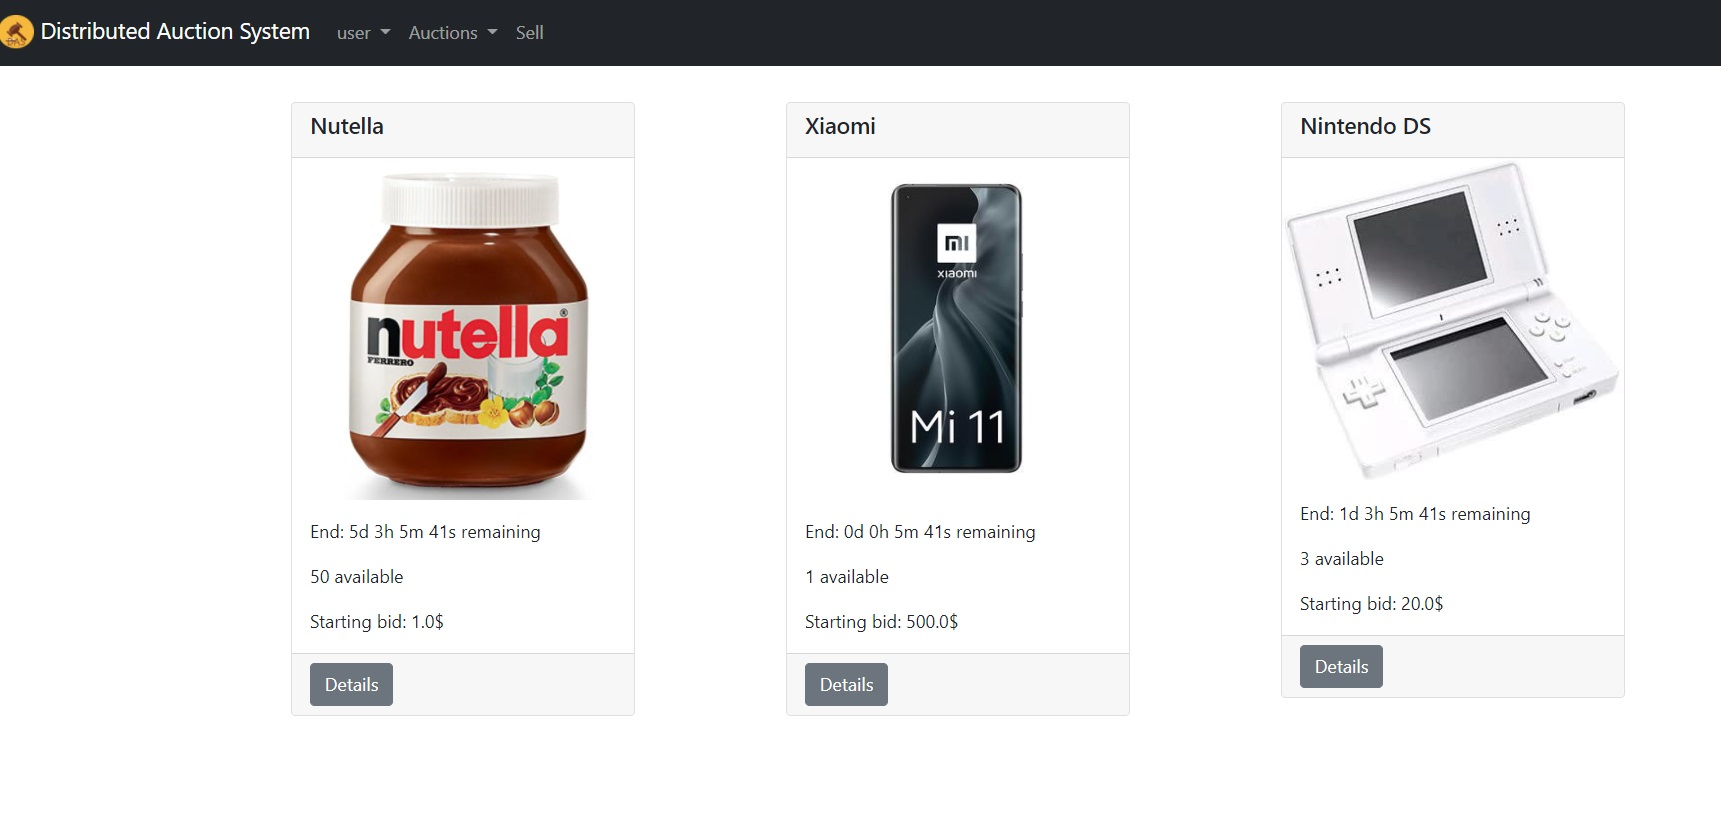
\includegraphics[width=\textwidth]{main-page}
	\caption{Application main page}\label{fig:main-page}
\end{figure}

\subsection{User Section}

\subsubsection{Modify Password}

To logout you have to click on the User section on the top page menu and then to
press ``Modify Password''. In the page shown in \figref{fig:modify} insert your
old password and then insert twice the new password that you desired. Then,
click on the button ``Modify''. You will see a message that says if the
operation is done correctly or not. If no error occurs, you can return to the
home page clicking on the button ``Home''.

\begin{figure}[htb]
	\centering
	%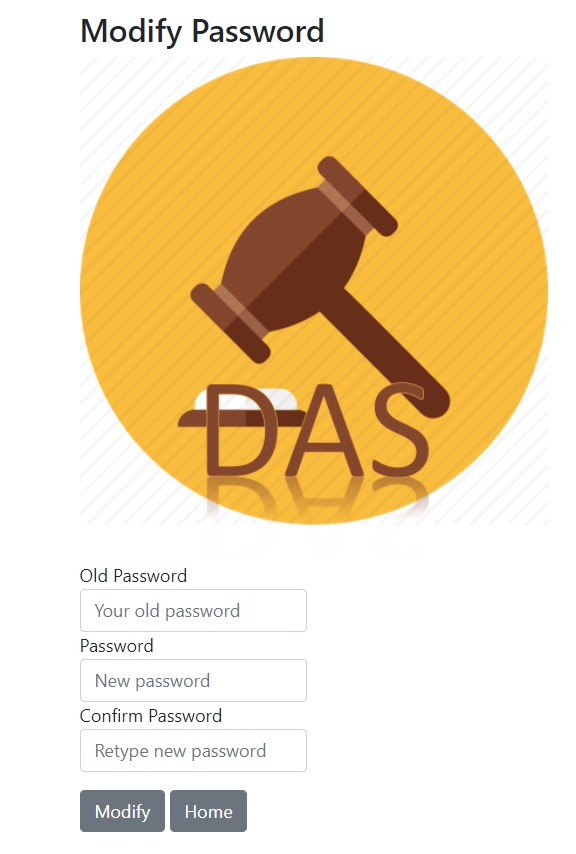
\includegraphics[width=\textwidth]{modify}
	\caption{Modify Password page}\label{fig:modify}
\end{figure}

\subsubsection{Logout}
To logout you have to click on the User section on the top page menu and then to
press ``Logout''. Now, if all is done correctly, you will see again the Login
page.

\subsection{Auctions Section}

%Auction List gia' descritta all'inizio

\subsubsection{MyAuctions}

\subsubsection{MyOffers}

\subsubsection{Select Auction}

%descrivere differenza fra bidder e agent selection

\subsection{Sell Section}

To create a new auction you have to click on the Sell section on the top page
menu. You are redirected to a page where you have to fill out a form, writing
the name of the auction, the minimum bid and the minimum raise you accept for
that auction, the number of items you want to sell for this auction, the date
and time you want the auction to end and a description of the items. It is also
necessary to upload an image of the items for sale. Then, click on the button
``Sell''. If no errors are shown, you have created a new auction.

\begin{figure}[htb]
	\centering
	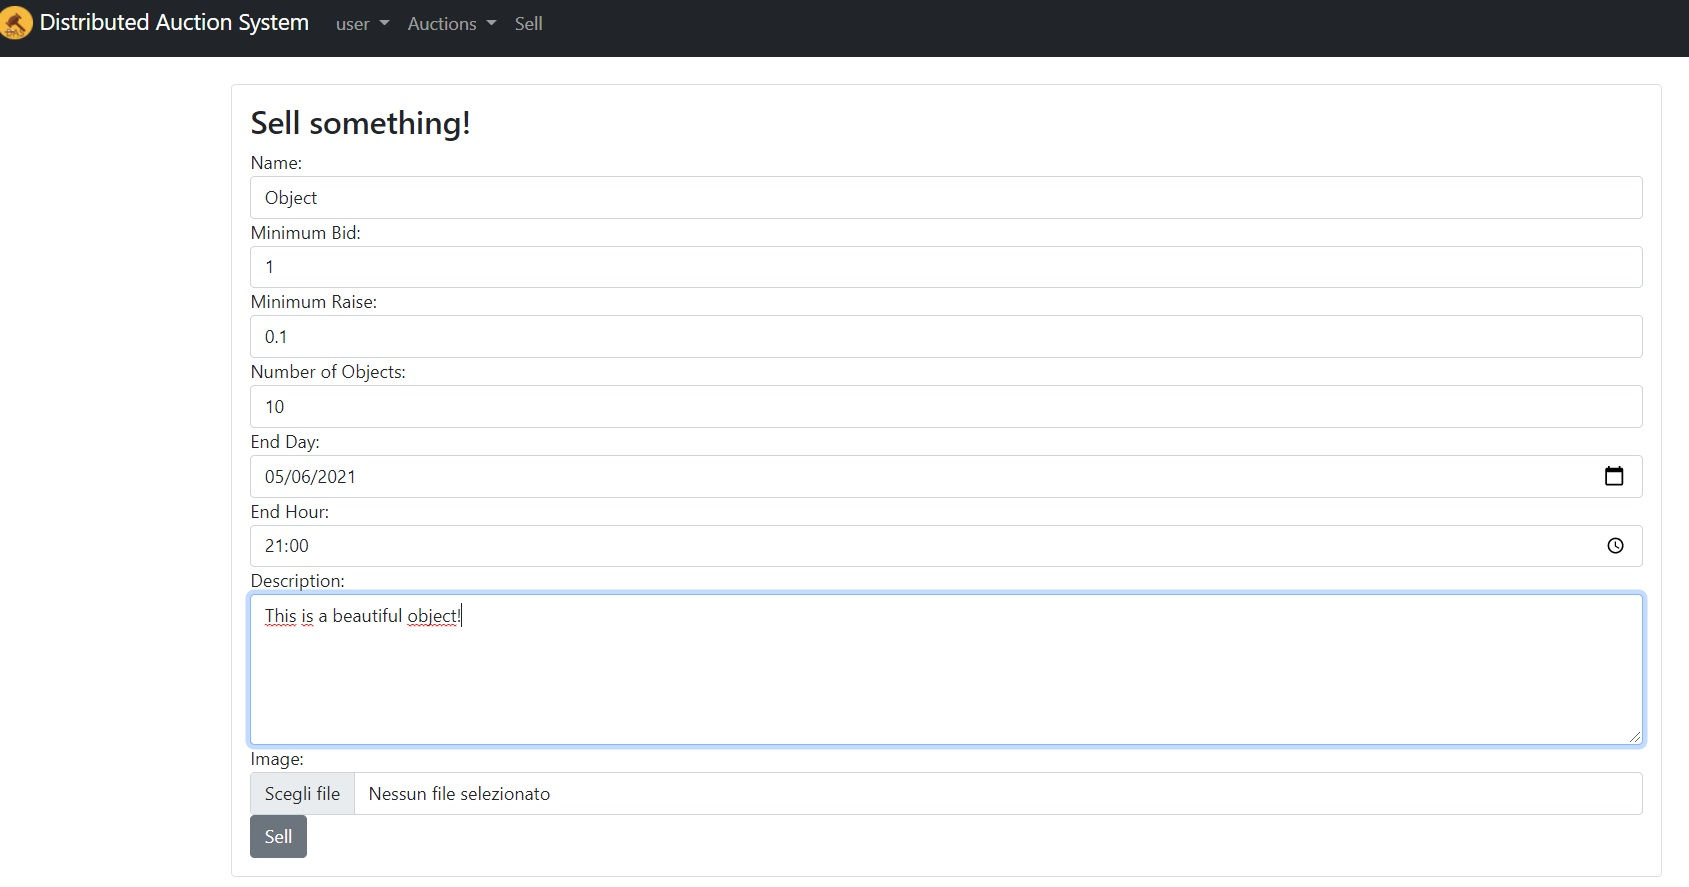
\includegraphics[width=\textwidth]{img/sell.jpg}
	\caption{Creation of a new auction}\label{fig:create-auction}
\end{figure}
